\chapter{Analytisk Mekanik}\label{cha:Mekanik}
\section{Newtons 2. lov og bevægelsesligninger} \label{sec:fjeder}
Hovedformålet med klassisk mekanik er at undersøge systemer i vores verden, specifikt at kunne beskrive bevægelser og interaktioner, som vi ser dem.
Newtons love, specielt hans 2. lov\footnote{Her er den skrevet på vektorform, men det betyder bare, at den gælder for hvert koordinat i det koordinatsystem, man vælger at benytte.}
\begin{align} \label{eq:N2}
	\sum\v{F} = m\v{a} = m\ddt{\v{r}} \: ,
\end{align}
lægger den grundlæggende byggesten for, hvordan klassiske problemer i mekanik løses. Beskrevet med ord siger ligning \eqref{eq:N2}, at summen af alle kræfter på et legeme, er det samme som legemets masse gange legemets acceleration, men hvordan bruger man det til vores formål, nemlig at kunne beskrive objekters bevægelse? For at svare på dette tages udgangspunkt i kraftanalyse og et eksempel med et lod på en fjeder. \\

\begin{figure*}[h!]
	\centering
	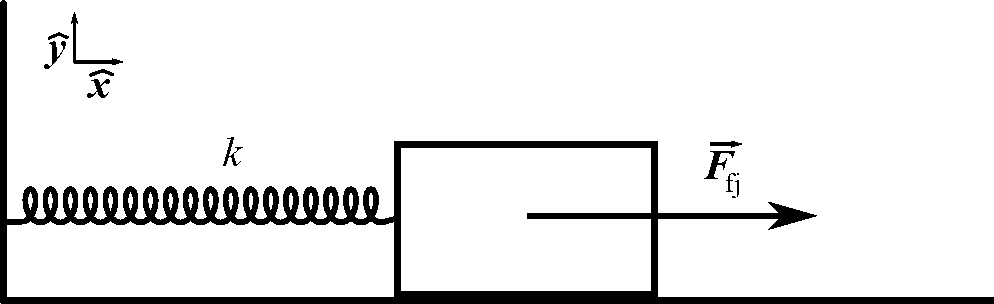
\includegraphics[width=.75\textwidth]{Analytisk-Mekanik/Fjeder.pdf}
	\caption{En klods, med massen $m$, fastspændt på en fjeder, med fjederkonstant $k$, hvor det hele er på en friktionsløs overflade. På tegningen er fjederen sammenpresset, hvorfor fjederen påvirker klodsen med en kraft, $\v{F}_\mathrm{fj}$, i den viste retning. Enhedsvektorerne i venstre hjørne viser at $x$-aksen er vandret, og $y$-aksen er lodret.} \label{fig:fjeder}
\end{figure*}
%
På figur \ref{fig:fjeder} ses en illustration af en fjeder fastspændt på en klods, hvor overfladen som klodsen bevæger sig på er friktionsløs. Fjederen har fjederkonstanten $k$ og klodsen har massen $m$. Her ses bort fra alle former for friktion, hvilket betyder at fjederkraften er den eneste kraft, der virker på klodsen. Inden dette problem løses, er det værd at overveje, hvilken løsning der forventes at få. Når fjederen er presset sammen, vil den forsøge at udvide sig, og når den er udstrakt, vil den forsøge at trække sig sammen. Det betyder, at klodsen svinger frem og tilbage omkring et ligevægtspunkt. Det forventes også, at udsvinget har en maksimal værdi samt at bevægelsen er periodisk, det vil sige at bevægelsen gentager sig. Her defineres koordinatsystemet således at klodsen i sin hvileposition er i $x = 0$, hvorved klodsens bevægelse kan beskrives med en sinus- eller cosinusfunktion, og her vælges cosinus\footnote{Havde man valgt sinus, ville det bare ændre værdien af $\delta$ med $\pi/2$. Pr. konvention vælges ofte cosinus, hvorfor det samme gøres her.} på formen
%
\begin{align} \label{eq:FjederSted}
	x(t) = A\cos(\omega t + \delta) \: ,
\end{align}
%
hvor $t$ er tiden, og $A$, $\omega$ og $\delta$ er konstanter. Cosinusfunktionen svinger mellem $-1$ og $1$, hvorfor $A$ er den maksimale afstand fra $x=0$, som klodsen kan have. $\omega$ er vinkelfrekvensen, og den hænger sammen med, hvor hurtigt klodsen svinger frem og tilbage. Fjederkonstanten $k$ er et udtryk for, hvor "hård"\;fjederen er, eller hvor meget energi det kræver, at presse fjederen sammen, mens massen $m$ er et mål for, hvor meget der skal til, for at ændre klodsens bevægelse. En logisk forventning ville derfor være, hvis $\omega$ på en eller anden måde afhænger af $k/m$. $\delta$ er en faseforskydningskonstant, og dens betydning ses ved at kigge på funktionen til tiden $t=0$. Her bliver $x(0) = A\cos\delta$, hvorfor $\delta$ er et udtryk for, hvor lodet er til tiden $t=0$. Cosinus er en periodisk funktion, der svinger frem og tilbage, hvorfor det giver mening at kunne beskrive klodsen på den måde. \\

At ligning \eqref{eq:FjederSted} faktisk beskriver klodsen, vil vi nu vise. Klodsen vil opleve en fjederkraft, $F_\mathrm{fj} = -kx$, som afhænger af fjederens forskydning fra dens ligevægtspunkt, hvilket kaldes  opførsel efter Robert Hooke. Det at fjederkraften har den form, er der ingen dybere teoretisk grund for, men det skyldes at eksperimenter viser, at fjedre kan beskrives på den måde, hvis de ikke deformeres.\footnote{Fjederkraften stiger jo mere der trækkes eller skubbes til fjederen, men trækker man for meget i fjereden, strækkes den så meget, at den holder op med at opføre sig som en fjeder. Her ses kun på tilfældet hvor $x$ ikke bliver så stor at fjederen ødelægges.} Det er antaget, at fjederkraften er den eneste i systemet, hvorfor Newtons 2. lov i 1 dimension giver, at $-kx = ma$, hvor $m$ er klodsens masse. Accelerationen $a$ er netop positionen af klodsen differentieret 2 gange med hensyn til tiden, $a = \dif[2]{t}{x}$ (differentieres et koordinat mht. tiden benyttes priknotationen, $\dif{t}{x} = \dt{x}$ og for dobbeltafledt $\ddt{x}$, fremover). Dette betyder, at vi faktisk har en 2. ordens differentialligning, der relaterer variablen $x$ til dens dobbeltafledte $\ddt{x}$
%
\begin{align} \label{eq:FjederDiffLign}
	m\ddt{x} = -kx.
\end{align}
%
Det særlige ved Newtons 2. lov er, at den giver os mulighed for, på en let og simpel måde, at opskrive de bevægelsesligninger (differentialligninger), som vi skal løse, for at kunne beskrive vores system. En beskrivelse af differentialligninger, kan findes i matematikafsnittet i appendiksetet, afsnit \ref{sec:difflign}. I modsætningen til almindelige ligninger, hvis løsninger er tal, så er løsningen til differentialligninger funktioner, og det er i matematikafsnittet bliver det forklaret, at differentialligninger kan være komplicerede at løse. Det er dog en hel del simplere at vise, at en funktion er en løsning til en differentialligning, end at finde en generel løsningsform dertil. At et tal er en løsning til en almindelige ligning, kan eftervises ved at sætte tallet ind på den ubekendtes plads, og så eftervise at ligningen går op. Det samme kan gøres med differentialligninger, hvor det så er funktionen, der indsættes. Det blev påstået at ligning \eqref{eq:FjederSted} beskriver klodsen, og derfor prøver vi nu at indsætte det i differentialligningen, ligning \eqref{eq:FjederDiffLign}. For at gøre det skal den dobbelt tidsafledte bestemmes
%
\begin{equation}
\begin{aligned}
	\ddt{x} &=\dif[2]{t}{}\left(A\cos(\omega t +\delta) \right) \\
	&= \dif{t}{}\left( -\omega A \sin(\omega t + \delta) \right) \\
	&= -\omega ^2 A \cos(\omega t + \delta ) \\
	&= -\omega^2x \: ,
\end{aligned}
\end{equation}
%
og indsættes det i ligning \eqref{eq:FjederDiffLign} fås
%
\begin{align}
	m(-\omega^2x) &= -kx \nonumber\\
	\implies \omega^2 &= \frac{k}{m} \: .
\end{align}
%
Her ses det at ligning \eqref{eq:FjederSted} opfylder ligning \eqref{eq:FjederDiffLign}, hvis $\omega^2 = k/m$. Med et snakkeargument fandt vi frem til, at $\omega$ måtte afhænge af $k/m$, og den præcise afhængighed er her opnået. Dette illustrerer at alt information, om hvordan et system opfører sig, er indeholdt i de differentialligninger, der kan opskrives ud fra Newtons love. Det kræver bare lige at de kan løses, hvilket eksempelvis kan gøres som her, ved at have et kvalificeret bud og så prøve efter, om det rent faktisk er en løsning. Man kan i nogle tilfælde bruge integration til at løse differentialligninger, hvilket kaldes separation af de variable. Ellers må man slå løsninger op eller finde numeriske løsninger med en computer.\footnote{Numeriske løsninger findes ved at sætte en computer til at regne en masse punkter, ud fra differentialligningen, til at forudsige opførslen af et bestemt system. Dette gøres tit, hvis der ikke kan laves fornuftige approksimationer til et system, eller for at teste fornuftigheden af de approksimationer man har lavet.} \\

%I vores nuværende problem med det skrå kast tager vi dog kun højde for én kraft, nemlig tyngdekraften, som i vores tilfælde er konstant $F_g = m\cdot g$, og altid rettet nedad mod jorden (dvs. i -y retningen). Da vi arbejder i to dimensioner giver dette os to rigtig simple differentialligninger, når vi anvender Newtons 2. lov:
%\begin{align}
%	F_{x,res} &= 0 = m\cdot \ddt{x} \\
%	F_{y,res} &= -m\cdot g = m\cdot \ddt{y}.
%\end{align}
%Dvs. at for det første ved vi ved reduktion af den første ligning, at $a_x = \ddt{x} = 0$, og for det andet ved vi, at $a_y = \ddt{y} = -g$. Altså at accelerationen i y-retningen er konstant -g, og at accelerationen i x-retningen er konstant 0. \\
%Nu har vi så vores to differentialligninger: hvad så? Hvordan løser vi dem så? \\
%Nu har vi jo allerede en ide om, hvordan vores bevægelse skal se ud, så lad os prøve med de tidligere nævnte udtryk for $x(t)$ og $y(t)$. \\

%Hvis $y(t) = v_{0,y} \cdot t - \frac{1}{2} \cdot g \cdot t^2$ differentieres 1 gang med hensyn til tiden får vi $v_y(t) = \dt{y} = v_{0,y} - g\cdot t$. Hvis vi gør det en gang til får vi $a_y(t) = \ddt{y} = -g$ netop som vores differentialligning giver os. Hvis vi gør det samme med $x(t) = v_{0,x}\cdot t$ får vi først $v_x(t) = \dt{x} = v_{0,x}$ og dernæst $a_x(t) = \ddt{x} = 0$, også i overensstemmelse med vores differentialligning. \\
%Derved er vi altså sikre på, at vi godt kan beskrive vores skrå kast ud fra de allerede kendte relationer for $x$ og $y$. \\ 
%
Det kan måske virke lidt som spildt arbejde at benytte differentialligningerne, hvis man kan gætte sig til en funktion, der beskriver systemet. Det svarer lidt til, at det i nogle tilfælde er ganske praktisk, at kunne gætte sig til en løsning til en almindelig ligning, men den metode afhænger af, at man har et godt gæt. Derfor er det smart at have en metode til faktisk at løse problemet, uden at skulle gætte sig frem. \\

Det skal vise sig fremadrettet at være en rigtig smart og sikker fremgangsmåde først og fremmest at finde differentialligningerne (eller nærmere bevægelsesligningerne) for ens system, hvis man ikke kender bevægelsesligningerne på forhånd. For hvis man kan finde bevægelsesligningerne, så er det eneste man mangler, nemlig at løse differentialligningen, hvor man ofte kan lave nogle simplificerende antagelser, hvis løsningen ikke er oplagt.

\section{Koordinater generelt}
I matematikafsnittet med polære koordinater, afsnit \ref{sec:PolKoord}, blev et relevant eksempel på et anderledes koordinatsystem end de kartesiske koordinater ($x,y,z$ koordinater) gennemgået, som kan være en fordel at benytte til at beskrive sit system. Indenfor mekanik er det netop denne tilgang, man har til koordinatsystemer. Man benytter dem som et redskab, til at beskrive sit system bedst og lettest muligt. Der er ikke en dybere fortolkning af ens valg af koordinater. \\

For eksempel kan et to-dimensionelt system beskrives med to rumlige, kartesiske, koordinater, $x$ og $y$. Hvis det vurderes fordelagtigt, i stedet at beskrive systemet med tre eller flere koordinater, så er man velkommen og indenfor al ret til at gøre dette. Dog mindskes kompleksiteten af et problem oftest ved at begrænse mængden af koordinater anvendt til den mindst nødvendige mængde. Ethvert almindeligt klassisk problem kan altid beskrives ud fra tre rumlige dimensioner per objekt/legeme i systemet. 
Generelt er et valgt koordinatsystem udtryk for, hvor mange dimensioner det forventes, at der skal bruges for nøjagtigt at beskrive problemet. Dette hænger tit sammen med, hvor mange retninger det forventes at et legeme kan bevæge sig i, totalt uafhængigt af andre retninger. Eksempelvis kan to uafhængige variable $a$ og $b$, samt en variabel $f(a,b)$ betragtes. At $a$ og $b$ er uafhængige af hinanden betyder her, at hvis værdien af $a$ ændres, så ændres værdien af $b$ ikke, og omvendt. Modsat er $f(a,b)$ afhængig af både $a$ og $b$, og kan derved ikke kaldes en uafhængig variabel. Ofte støder man på variable, der er implicit afhængige, hvilket betyder at man ikke skriver (eksplicit) at variablen afhænger af en anden. Dette ses tit med koordinater, hvor man ofte skriver eksempelvis $x$ i stedet for $x(t)$, idet man antager det for kendt, at $x$ afhænger af $t$. Dette er vigtigt, da man ønsker at beskrive systemet med så få uafhængige koordinater som muligt. \\ % Dette er uklart i forhold til tidsafhængighed og frie variable. Der skelnes ikke her mellem frie variable som t, og de variable vi finder udtryk for til at beskrive vores system (som afhænger af enten t eller en anden tidsafhængig variabel).
%

At koordinatsystemet her betragtes som givende udtryk for det \textit{forventede} antal uafhængige bevægelser, forklares ud fra, at det ikke altid kan vides på forhånd, hvorvidt en variabel er afhængig af andre variable eller ej. Dette finder man ud af, når man analyserer systemet, som man har med at gøre, hvorefter man kan tilrette sine koordinater efter det. Som eksempel på dette tages et simpelt pendul, som vi vil analysere senere. Umiddelbart kan pendulets bevægelse beskrives ud fra to kartesiske koordinater, $x$ og $y$, der varierer i tiden $t$, eller alternativt med to polære koordinater, med en vinkel $\phi$ og en pendullængde $r$, der også begge varierer med tiden. I dette tilfælde viser det sig dog, at længden $r$ er konstant og ikke variabel, hvormed systemet burde kunne beskrives udelukkende ud fra et udtryk for vinklen $\phi$ til tiden $t$. Men hvad med de to kartesiske koordinater $x$ og $y$? Her kan det senere vises, at den ene af de to koordinater er overflødige, da der kan findes et funktionsudtryk, som beskriver pendulets bevægelse i den ene retning ud fra dens bevægelse i den anden. Dette er dog ikke altid tilfældet, hvormed det giver god mening, at starte ud med begge koordinater. Herefter kan man altid fjerne koordinater, der ikke er nødvendige, ved ændre på sit koordinatsystem. \\

Som det vil blive nævnt senere i afsnittet om generaliserede koordinater, så er det smart at vælge sine koordinater, efter at man har gjort sig nogle indledende overvejelser omkring sit system, for at begrænse den opfattede kompleksitet af ens system. Tit vil ens system nemlig have symmetrier eller lignende restriktioner i sin bevægelse, som så vil sætte begrænsninger på antallet af koordinater (senere nævnt som frihedsgrader), der er nødvendige for at beskrive systemet. Dette bliver anvendt til, at løse de fleste af problemerne I bliver præsenteret for i dette kapitel, samt i de andre kapitler, specielt kapitlet om planetbevægelse. Udover at nævne pendulet som eksempel igen, er det dog værd at nævne, at mange systemer, med to legemer, har disse begrænsninger, og flere endda kan reduceres til kun at have en variabel (i stedet for to til hvert legeme), hvormed hele systemets bevægelse kan beskrives ved bare at kende en enkelt værdi.

\section{Roterende legemer}
Legemers bevægelse kan, i den Newtonske mekanik, deles op i to kategorier - translatorisk og rotationel bevægelse. Her menes bevægelse med og uden rotation. Vi starter med at se på den rotationelle del af legemers bevægelse, hvor der vil fokuseres på stive legemer, hvilket vil sige faste objekter, der ikke kan bøje eller deformeres. Beskrivelsen af legemers bevægelse deles op i tre dele - kinematik, energi og dynamik. Kinematik er beskrivelsen af legemers bevægelse, når bevægelsens oprindelse ikke tages med i betragtning. Dynamik beskriver hvorfor ting bevæger sig som de gør, og hvordan kinematiske bevægelser opstår. Det viser sig at energi er en vigtig størrelse at undersøge, når man skal beskrive bevægelse, hvorfor vi vil kigge på energien i både translatorisk og rotationel bevægelse.

\subsection{Kinematik}
I den translatoriske bevægelse beskrives et legemes position med en stedvektor $\v{r}$, der kan udtrykkes i forskellige koordinatsystemer. I det kartesiske koordinatsystem ser vektoren ud på en af følgende måder
%
\begin{align*}
	\v{r} = \xyz{x}{y}{z} = x\xhat + y\yhat + z\zhat \: ,
\end{align*}
%
hvilket betyder at legemet befinder sig i punktet $(x,y,z)$. Ud fra stedvektoren defineres hastighed $\v{v}$ og acceleration $\v{a}$ som\footnote{Man kan selvfølgelig differentiere stedvektoren ligeså mange gange man lyster, og selvom højere afledede bruges meget sjældent, har de faktisk nogle navne (på engelsk), som man kan underholde sig selv ved at google. Den tredjeafledede $\d^3\v{r}/\d t^3$ er dog værd at fremhæve, da den på engelsk hedder "jerk".}
\begin{equation}
    \v{v} \equiv \dt{\v{r}} \: , \qquad \v{a} \equiv \ddt{\v{r}}.
\end{equation}
%
\begin{figure}[h!]
\centering
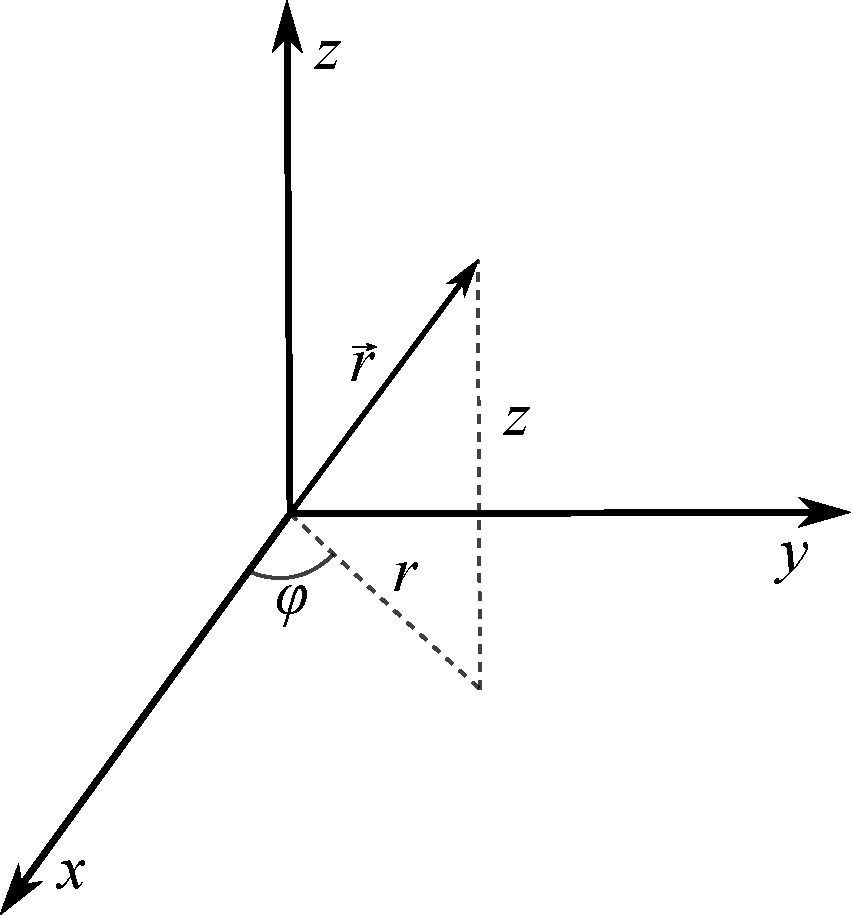
\includegraphics[width=.4\textwidth]{Analytisk-Mekanik/CylindriskeKoordinater}
\caption{I det cylindriske koordinatsystem angives afstanden til $z$-aksen som første koordinat, samt forskydningen langs samme akse som $z$-koordinat. Derudover angives vinklen med polæraksen, her ækvivalent med $x$-aksen. $z$-koordinatet er derved det samme i det kartesiske og cylindriske koordinatsystem.}
\label{fig:CylindriskeKoordinater}
\end{figure}
%
%
\subsubsection{Cylindrisk polære koordinater}
Til beskrivelsen af roterende legemer benyttes ofte cylindriske koordinater i stedet for kartesiske koordinater. Cylindriske koordinater er en tredimensionel udvidelse af de todimensionelle polære koordinater, hvor 3. koordinatet, $z$, forskyder punktet parallelt med en akse, der er ortogonal (vinkelret) på den todimensionelle plan udspændt af de polære koordinater, gennem origo, (0,0,0). I polære koordinater defineres et punkt  som origo, og ud fra det en polærakse, der angiver placeringen af vinklen på $\phi = 0$ radianer. Et punkts afstand til origo, $r$, og dets vinkel med polæraksen, $\phi$, angiver så de polære koordinater. Defineres koordinatsystemet således at polæraksen og $x$-aksen i et tilsvarende kartesisk koordinatsystem er sammenfaldende, ville $\phi$ være vinklen ift. $x$-aksen i $xy$-planen og $z$ er forskydningen ift. polærplanen, se figur \ref{fig:CylindriskeKoordinater}. Det bemærkes, at det kartesiske 3. koordinat og det cylindriske 3. koordinat er ens, og at afstanden $r$ ved udvidelsen fra polære til cylindriske koordinater forbliver uændret; det vil sige at en ændring i $z$ ikke giver en ændring i $r$. Da der kun fokuseres på legemers rotation om én akse, kan $z$-aksen defineres til at være denne rotationsakse, hvorved det cylindriske 3. koordinat forbliver uændret i tid.  \\

I polære koordinater er der en meget nyttig sammenhæng mellem et legemes totale fart og den tidsafledte af vinkelkoordinatet $\dt{\phi}$. Det antages at førstekoordinatet, $r$, er konstant i tid, $\dt{r} = 0$. Derfor kan ligning \eqref{eq:kartesisk/polaer} fra matematikafsnittet\footnote{I matematikafsnittet hedder vinklen $\theta$, hvor den her hedder $\phi$. Det betyder ikke det store hvad man kalder den, men her i kapitlet bruges $\phi$, hvor denne notation bruges konsekvent.} benyttes til at opskrive de tidsafledede af de kartesiske koordinater udtrykt ved de polære koordinater
%
\begin{equation}
\begin{aligned}
	\dt{x} &= -r\sin\phi\dt{\phi} \: , \\
	\dt{y} &= r\cos\phi\dt{\phi} \: .
\end{aligned}
\end{equation}
%
Da hastighed er en vektor, $\v{v} = \dot{x} \xhat + \dot{y} \yhat$, så er den totale fart længden af hastighedsvektoren, og den kan bestemmes vha. Pythagoras sætning
%
\begin{equation} \label{eq:SmartFart}
\begin{aligned}
	v &= \sqrt{\dt{x}^2 + \dt{y}^2} \\
	&= \sqrt{(-r\sin(\phi)\dt{\phi})^2 + (r\cos(\phi)\dt{\phi})^2} \\
	&= \sqrt{r^2\dt{\phi}^2(\cos^2\phi + \sin^2\phi)} \\
	&= r\dt{\phi}\sqrt{\cos^2\phi + \sin^2\phi} \\
	&= r\dt{\phi} \: .
\end{aligned}
\end{equation}
%
Her er grundrelationen $\cos^2\phi + \sin^2\phi = 1$ benyttet, og dette resultat bliver super anvendeligt, når der skal bestemmes energier for roterende legemer, hvilket er en essentiel del af Lagrangemekanikken, som kommer senere. Differentieres ligning \eqref{eq:SmartFart} igen med hensyn til tid fås
\begin{align}
	a = r\ddt{\phi} \: .
\end{align}

\subsubsection{Vinkelhastighed og Vinkelacceleration}
%
\begin{figure}[h!]
\centering
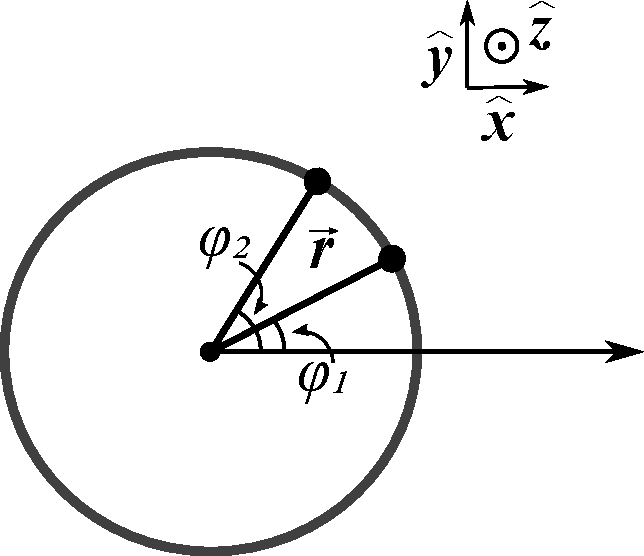
\includegraphics[width=.4\textwidth]{Analytisk-Mekanik/Roterende-Legeme}
\caption{Til to forskellige tider har det sorte punkt to forskellige vinkler med polæraksen (markeret med pil), der her er sammenfaldende med den kartesiske $x$-akse, mens legemet roterer om $z$-aksen. $\v{r}$ er en vektor fra origo til punktet, og har derfor længden $r$ og vinklen $\phi$ med polæraksen. Denne vektor ændrer sig i tid, som punktet flytter sig.}
\label{fig:Roterende-Legeme}
\end{figure}
%
Figur \ref{fig:Roterende-Legeme} viser hvordan vinklen $\phi$ ændrer sig fra tidspunktet $t_1$ til $t_2$. Helt analogt til den translatoriske bevægelse defineres vinkelhastigheden, $\omega$, og vinkelacceleration, $\alpha$, som
%
\begin{equation}
    \omega\equiv\dt{\phi} \: , \qquad \alpha\equiv\dt{\omega}=\ddt{\phi} \: .
\end{equation}
%
Vinkelhastigheden er et udtryk for, hvor hurtigt et legeme roterer og har enheden $\si{\radian/\second}$. Vinkelaccelerationen udtrykker, hvor hurtigt rotationshastigheden ændres i enheder af $\si{\radian/\second\squared}$. Her er "$\si{\radian}$"\;symbolet for enheden radianer.

\subsubsection{Inertimomentet}
Eksperimenter viser, at et legemes modstand mod acceleration ikke kun afhænger af legemets masse, men også placeringen af massen, hvorfor inertimomentet for et objekt defineres som\footnote{Symbolet $\equiv$ betyder indenfor fysik \textit{defineres som}, hvor $:=$ benyttes i matematik.}
%
\begin{equation} \label{eq:Inertimoment}
    I \equiv \sum m_ir_i^2 \: ,
\end{equation}
%
hvor $m_i$ er massen af det $i$'te masseelement og $r_i$ er samme masseelements afstand til rotationsaksen. Ethvert legeme kan tænkes som bestående af en masse små dele, kaldet masseelementer, og inertimomentet udtrykker så hvor langt fra rotationsaksen et legemes masse er placeret. Definitionen er en smule rigid, men en konceptuel forståelse er tilstrækkelig her. $I$ afhænger af den akse, som legemet  roterer om, hvilket kan forklares ved at legemer lettere kan sættes i rotation om bestemte akser end andre. Dette kan man afprøve ved at tage et objekt og prøve at rotere det på forskellige måder. Man vil mærke at nogle rotationer er lettere end andre.


\subsection{Kinetisk Energi}
For translatorisk bevægelse defineres kinetisk energi som
%
\begin{equation} \label{eq:Ktrans}
    K_{\text{trans}}=\frac{1}{2}mv_\textsc{cm}^2 \,,
\end{equation}
%
hvor $v_\textsc{cm}$ er massemidtpunktets fart. Hvis hele legemet bevæger sig med samme fart $v$ er $v_\textsc{cm} = v$, men hvis legemet eksempelvis roterer, bevæger forskellige dele af legemet sig med forskellige hastigheder. \\
Rotationskinetisk energi defineres tilsvarende som
%
\begin{equation} \label{eq:Krot}
    K_{\text{rot}}=\frac{1}{2}I\omega^2 .
\end{equation}
%
Bemærk at ligningerne \eqref{eq:Ktrans} og \eqref{eq:Krot} har præcis sammen form, idet energien i begge tilfælde er proportional med en form for inerti og en fart i anden. Den totale kinetiske energi for et roterende legeme er summen af de to ovenstående
%
\begin{equation} \label{eq:K}
    K_{\text{tot}}=K_{\text{trans}}+K_{\text{rot}} \: .
\end{equation}
%
At den totale kinetiske energi "bare"\;er summen af translatorisk og rotationel kinetisk energi, bør man strengt taget vise, men det er en smule omstændigt, hvorfor det undlades her.

\subsection{Dynamik}
%
\begin{figure}[h!]
\centering
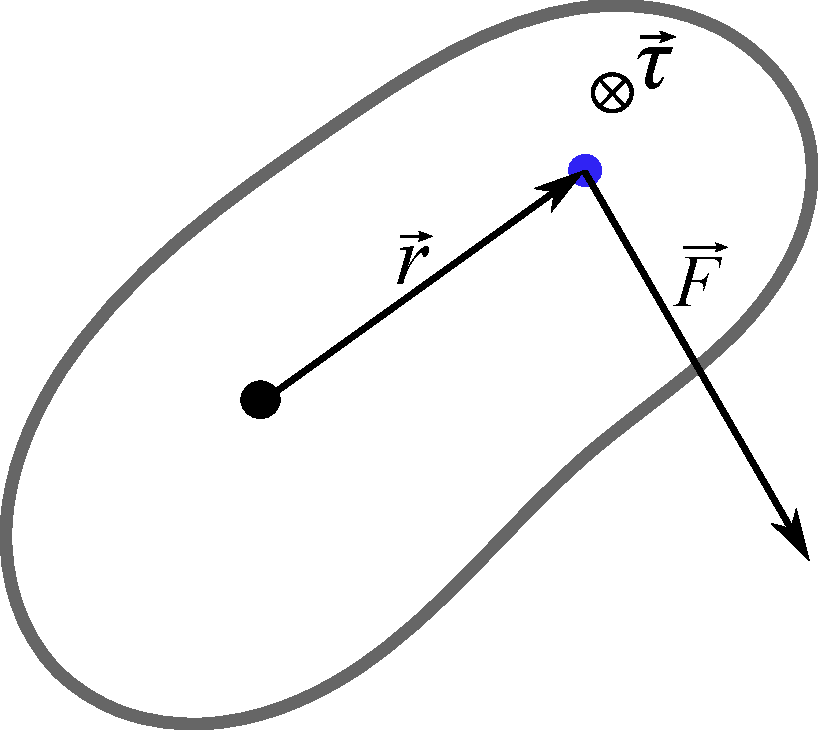
\includegraphics[width=.4\textwidth]{Analytisk-Mekanik/Kraftmoment}
\caption{En arbitrær kraft, $\v{F}$, virker i det blå punkt, hvorfor dette punkt kaldes kraftens angrebspunkt. Legemet roterer om en akse gennem det sorte punkt, der er ortogonal på tegningen. Det sorte punkt kan defineres som origo, hvorved vektoren fra rotationsaksen til kraftens angrebspunkt kaldes kraftens arm $\v{r}$. Kraftmomentet $\gv{\tau}$ peger ind i tegningen, hvilket højrehåndsreglen viser.}
\label{fig:Angrebspunkt}
\end{figure}
%
Kræfter er årsagen til bevægelse, som det kendes i fysik, og med hensyn til den translatoriske bevægelse er det ikke essentielt, hvor på legemet kraften virker, men det er det for rotationel bevægelse. Der findes mange dagligdags eksempler på dette, hvor et af de bedre er et værktøj, som en svensknøgle, der holder om en bolt. Jo længere nede på svensknøglen man holder, desto lettere er det at stramme eller løsne bolten. For at forstå fysikken bag dette, introduceres angrebspunktet for kraften $\v{F}$ som det punkt på et legeme, hvorpå kraften virker, se figur \ref{fig:Angrebspunkt}. Yderligere defineres en vektor fra rotationsaksen til kraftens angrebspunkt, hvilket kaldes kraftens arm $\v{r}$. Herved kan kraftmomentet, $\v{\tau}$, defineres
%
\begin{equation} \label{eq:Kraftmoment}
    \v{{\tau}} \equiv \v{r}\times\v{F} \: .
\end{equation}
%
Kraftmomentet er en vektor, der står ortogonalt på både kraften og dens arm, og den er parallel med rotationaksen. Kraftmomentets størrelse kan bestemmes som
%
\begin{equation} \label{eq:KraftmomentNorm}
\tau = rF\sin\theta \: ,
\end{equation}
%
hvor $\theta$ er vinklen mellem $\v{r}$ og $\v{F}$. Dette leder til Newtons 2. lov for roterende legemer
\begin{align}
	\sum\tau = I\alpha \: .
\end{align}
Det ville være super anvendeligt, hvis dette galt ligeså alment, som Newtons 2. lov, $\sum\v{F} = m\v{a}$, men det er desværre ikke tilfældet. Den gælder for legemer, der er symmetriske omkring rotationsaksen og kun for størrelsen af vektorerne.


%\begin{figure}[h!]
%\centering
%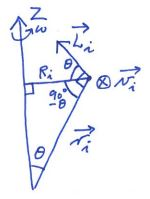
\includegraphics[width=.25\textwidth]{Analytisk-Mekanik/Impulsmoment}
%\caption{ Det $i$'te delelement af et arbitrær stift legeme, med hastighed og impulsmoment som vist, hvor kraftens arm er defineret ud fra et punkt på rotationsaksen.}
%\label{fig:Impulsmoment}
%\end{figure}

\subsubsection{Impulsmoment}
Impulsmomentet defineres ud fra den lineære impuls $\v{p}=m\v{v}$ som
%
\begin{equation} \label{eq:L}
    \v{\ell} \equiv \v{r}\times\v{p} \: .
\end{equation}
%
Størrelsen på impulsmomentet er
%
\begin{equation}
	\ell = rp\sin\theta \: ,
\end{equation}
%
hvor $\theta$ er vinklen mellem $\v{r}$ og $\v{p}$. Differentieres ligning \eqref{eq:L} med hensyn til tiden fås
\begin{equation}
    \dt{\v{\ell}} = \dif{t}{}\left(\v{r}\times\v{p}\right) = \dif{t}{\v{r}}\times m\v{v}+\v{r}\times m\dif{t}{\v{v}} = \v{v}\times m\v{v}+\v{r}\times m\v{a} = \v{r}\times\sum\v{F} = \sum\gv{\tau} \: ,
\end{equation}
idet et krydsprodukt af to parallelle vektorer er nul. Det er da vist at
\begin{equation} \label{eq:sum_tau_lig_aflede_impulsmoment}
    \sum\gv{\tau} = \dt{\v{\ell}} \: .
\end{equation}
Det kan vises at summen af de indre kraftmomenter er nul, og impulsmomentet er da bevaret, hvis og kun hvis summen af de ydre kraftmomenter er nul.

\subsection{Newtonsk beskrivelse af et pendul} \label{sec: Beskrivelse af pendul - Newton}

\begin{figure}[t]
\centering
\begin{subfigure}{.45\textwidth}
  \centering
  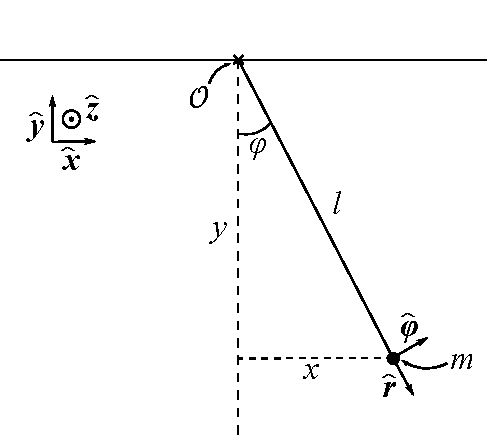
\includegraphics[width=\linewidth]{Analytisk-Mekanik/Pendul.pdf}
\caption{Skitsering af pendul med massen $m$ og længden $l$. Enhedsvektorerne til et kartesisk og cylindrisk polært koordinatsystem er indtegnet.}
\label{fig:Pendul}
\end{subfigure}
\hspace{5mm}
\begin{subfigure}{.45\textwidth}
  \centering
  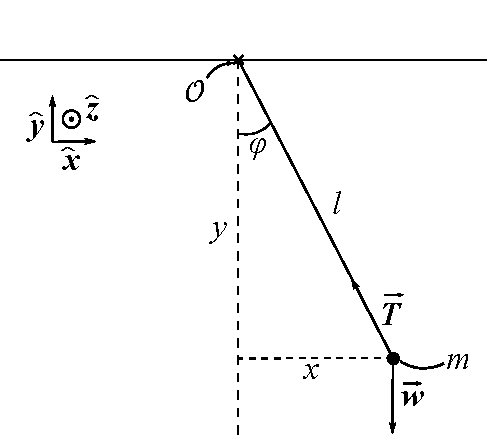
\includegraphics[width=\linewidth]{Analytisk-Mekanik/PendulKraft.pdf}
  \caption{Kraftanalyse af de på pendulloddet virkende kræfter, der alle antages at have angrebspunkt i massemidtpunktet.}
  \label{fig:Kraftanalyse}
\end{subfigure}
\caption{Tegning af pendulet, der blandt andet viser de valgte koordinatsystemer og de virkende kræfter.}
\end{figure}

I første omgang defineres et smart koordinatsystem til at beskrive pendulet. Som origo vælges pendulets ophængningspunkt, se figur \ref{fig:Pendul}. Pendulloddets position, til tiden $t$, beskrives ved en retningsvektor i cylindrisk polære koordinater $\v{r}(r,\phi,z,t)$, hvor $r$ er lodets afstand til aksen gennem origo, $\phi$ er polærvinklen, og $z$ er forskydningen fra polærplanen. Det antages at pendulet bevæger sig i ét plan, hvilket defineres som $z=0$, hvorfor $z$ forbliver uændret når tiden går. Det antages yderligere at lodets ophængning er et stift, ubøjeligt legeme, hvorfor $r=l \enspace\forall t$ \footnote{$\forall$ er matematisk notation for \textit{for alle}.}. Pendulet kan under disse antagelser beskrives fuldstændigt ved vinklen $\phi$, hvorfor stedfunktionen, $\phi(t)$, er interessant at bestemme. Pendulet kan også beskrives ved kartetiske koordinater, hvilket er indtegnet i figur \ref{fig:Pendul}, og det har visse fordele i forhold til den intuitive forståelse af systemet, når kraftanalysen udføres. \\

\noindent
På pendulet virker tyngdekraften, $\v{w}$, og en snorkraft, $\v{T}$, se figur \ref{fig:Kraftanalyse}. Det er de eneste kræfter på pendulet, idet friktion negligeres.\footnote{Det er muligt at regne med friktion, men det komplicerer situationen en del.} Tyngdekraften virker til alle tider, $t$, i negativ $y$-retning og skrives derfor som
\begin{align}
	\v{w} = -mg\yhat \: ,
\end{align}
hvor $g$ er tyngdeaccelerationen, og $\yhat$ er en enhedsvektor i $y$-retningen. Det bemærkes at $\yhat$ er en kartesisk enhedsvektor.\footnote{Teknisk set er $\yhat$ en enhedsvektor i begge koordinatsystemer, idet en enhedsvektor er en vilkårlig vektor med længden 1. Det vigtige er her at det er en enhedsvektor i den kartesiske basis og ikke i den polære.} \\
Defineres $\boldsymbol{\hat{r}}$ som en enhedsvektor parallelt med pendulets retningsvektor, hvilket også er en enhedsvektor i det polære koordinatsystem, kan snorkraften beskrives som
\begin{align}
	\v{T} = -T\boldsymbol{\hat{r}} \: ,
\end{align}
hvor $T$ er størrelsen på snorkraften, som vist på tegningen. Dette betyder, at hver kraft er simplest at beskrive i to forskellige koordinatsystemer, og faktoren $T$ har lige præcis den værdi, som får systemet til at passe. Dette viser en af svaghederne ved den Newtonske beskrivelse af mekanik - håndteringen af "tvangskræfter", eller "constraint forces" på engelsk, er kluntet. \\

\noindent
Pendulet roterer omkring ophængningspunktet, og har ved denne rotation inertimomentet $I$. Alle kræfter antages at virke på loddets massemidtpunkt, hvorfor alle kræfters arm kan beskrives som
%
\begin{align}
	\v{r} = l\boldsymbol{\hat{r}} \: ,
\end{align}
%
hvilket også er pendulloddets stedvektor. Nu kan kraftmomentet for alle de virkende kræfter bestemmes
%
\begin{equation}
\begin{aligned}
	\gv{\tau}_w &= \v{r} \times \v{w} = -mg \cdot \boldsymbol{r} \times \yhat = -mgl\sin\phi\zhat \: , \\
	\gv{\tau}_T &= \v{r} \times \v{T} = -Tl \cdot \v{r} \times \v{r} = \v{0} \: ,
\end{aligned}
\end{equation}
%
hvor subscriptet indikerer, hvilken kraft der behandles. Det samlede kraftmoment bliver derved
%
\begin{align}
	\sum\gv{\tau} = - mgl\sin\phi \zhat \: .
\end{align}
%
Antages pendulets udsvingsvinkel at være lille, kan en andenordens Taylorudvikling benyttes
%
\begin{align}
	\sin\phi\approx\phi \implies \sum\tau \approx -mgl\phi \: ,
\end{align}
%
hvor Newtons anden lov for rotationel bevægelse giver differentialligningen
%
\begin{align}
	\ddt{\phi} = \frac{1}{I}\sum\tau = -\frac{mgl}{I}\phi \: .
\end{align}
%
Denne differentialligning har løsningen
%
\begin{align} \label{eq:PendulFuld}
	\phi(t) = A\cos\left(\omega t + \delta\right), \quad \omega^2 = \frac{mgl}{I} \: ,
\end{align}
%
hvor $A$ og $\delta$ er konstanter, der er bestemt af startbetingelserne. Eftersom cosinusfunktioner giver værdier mellem $-1$ og $1$, så er $A$ den maksimalen udsvingsvinkel og $\delta$ er en faseforskydning, så pendulet kan være et hvilket som helst sted i sit udsving til tiden $t=0$.
Dette medfører, at pendulets periode bliver
%
\begin{align}
	T = \frac{2\pi}{\omega} = 2\pi\sqrt{\frac{mgl}{I}} \: .
\end{align}
%
Slutteligt kan pendulets $x$-koordinat beskrives som
%
\begin{align}
	x(t) = l\sin\phi(t) \approx l\phi(t) \: ,
\end{align}
%
hvor der til sidst igen gøres brug af en andenordens Taylorudvikling. Denne beskrivelse af et pendul kaldes et \textit{fysisk pendul}.

\subsubsection*{Matematisk pendul}
Antages pendulets masse at befinde sig i pendulets massemidtpunkt kan inertimomentet sættes til $I=ml^2$ i ligningerne fra det fysiske pendul:
%
\begin{align} \label{eq:PendulLigning}
	\ddt{\phi} = -\frac{g}{l}\phi \: ,
\end{align}
%
hvorved løsningen bliver
%
\begin{align}
	\phi(t) = A\cos\left(\omega t + \delta\right), \quad \omega^2 = \frac{g}{l} \: ,
\end{align}
%
hvilket giver en periode på
%
\begin{align}
	T = \frac{2\pi}{\omega} = 2\pi\sqrt{\frac{l}{g}} \: .
\end{align}
%
Ligning \eqref{eq:PendulLigning} er pendulligningen og rigtig mange ting i fysik kan approksimeres til en harmonisk oscillator, dvs. beskrevet ved en bevægelsesligning, for et koordinat $q$, på formen
%
\begin{align}
	\ddt{q} = -\omega^2q \: ,
\end{align}
%
hvorfor denne ligning er værd at huske på. Loddet på en fjeder var et andet eksempel på en harmonisk oscillator.

\section{Generaliserede koordinater}
I eksemplet med pendulet fremgik det, at koordinaterne $r$ og $z$ var overflødige. De var konstante i tid ved valg af et smart koordinatsystem og hele pendulet kunne beskrives ved ét koordinat, $\phi$. Dette er en generel tankegang i analytisk mekanik, da der ikke er nogen grund til at gøre problemet sværere, end det allerede er. Man kan prøve at regne pendul-eksemplet igennem, kun ved brug af de kartesiske koordinater $x$ og $y$, og man opdager hurtigt, at det er meget besværligt. Derfor introduceres konceptet generaliserede koordinater, der defineres som det sæt koordinater, der beskriver et fysisk system med det mindst mulige antal frihedsgrader. Antallet af frihedsgrader er antallet af uafhængige parametre, som beskriver et system, hvilket for pendulet er 1. Generaliserede koordinater har symbolet $q$, samt et indeks $i$, der fortæller hvilket koordinat der er tale om. Grunden til dette er, at teorien gælder for systemer med vilkårligt mange frihedsgrader. Beskrives fire partikler, som bevæger sig i en dimension, kan partiklernes koordinat noteres som $(q_1,q_2,q_3,q_4)$ eller $(q_1,q_2,...,q_4)$. Den sidste notation er ikke så praktisk i dette eksempel, men da teorien skal kunne beskrive $n$ partikler, så bliver den pludselig smart, idet koordinaterne bliver
%
\begin{align}
	(q_1,q_2,...,q_n) \: .
\end{align}
%
Ønsker man at beskrive noget som gælder for alle $n$ partikler, hvilket f.eks. kunne være at hastigheden for partiklen er givet som den tidsafledte skriver man
\begin{align}
	v_i = \dt{q}_i \: , \quad \forall \, i=1,2,...,n \: .
\end{align}
Fremover benyttes notationen $q_i$ for det $i$'te generaliserede koordinat, idet der tages højde for, at der kan være vilkårligt mange af disse, og at det også kan være nødvendigt med flere generaliserede koordinater for at beskrive én partikel. \\

Kunsten at bestemme de generaliserede koordinater bygger mange gange på at kunne genkende symmetrier. Symmetrier gør problemer lettere at håndtere, og det er derfor altid en god idé at overveje, om der er sådanne for et fysisk system. I pendul-eksemplet er der tale om cirkulær symmetri. Antagelserne at $r$ og $z$ er konstante i tid, gør at pendulets bevægelse bliver restringeret til en cirkel, hvilket kan kaldes cirkulær symmetri.

\section{Lagrangefunktion}
Generelt er Newtons love gode i sin simplicitet, med let forståelse af dem og deres anvendelse. Dette gør dem essentielle til, at have en generelt løsningsmetode til de fleste problemer. En af ulemperne ved dem er dog, at problemløsningen ofte er en slavisk proces, der kræver at man tager højde for alle kraftpåvirkninger på ens system, og kan gøre systemet mere kompliceret end det er. Et eksempel på dette er systemer, hvis bevægelse har restriktioner fra snorkræfter, normalkræfter eller lignende, der ikke udfører arbejde på systemet. Her menes der, at netop disse "constrained forces"\;sætter begrænsninger på, hvordan systemet kan bevæge sig, men at de i sig selv ikke tilføjer eller fratager energi fra systemet.Newtons love kræver dog, at de inkluderes i udregningerne for at kunne beskrive systemet korrekt. \\

Her introduceres fordelen ved Lagrangemekanikken, der tager udgangspunkt i en undersøgelse af den kinetiske og potentielle energi i et system, samt en opskrivning af differentialligninger ud fra dette, ligesom for Newtonsk mekanik (Newtons 2. lov beskriver, hvordan man opsætter differentialligninger for systemet, da $\sum\v{F} = m\v{a} = m\ddt{\v{r}}$). Ulempen ved Lagrangemekanik, i formen der introduceres her er, at den kun gælder for systemer udelukkende påvirket af konservative kræfter. Dette inkluderer derved ikke gnidningskræfter, luftmodstand og lignende.  \\

\noindent Systemet undersøges ud fra en funktion kaldet Lagrangefunktionen:
\begin{align} \label{Lagrange_funktion}
	L = K - V,
\end{align}
hvor $K$ er systemets kinetiske energi, og $V$ er systemets potentielle energi.

\subsection*{Euler-Lagrangeligningen i kartesiske koordinater}
Først vil vi beskrive vores energier ud fra kartesiske koordinater i et inertialsystem, hvilket altid kan gøres, og derefter kan det konverteres over til mere favorable, generaliserede koordinater, som vælges specifikt for hvert system. Disse gør normalt problemet lettere at løse. Vi vil desuden tage udgangspunkt i et system uden bundne kræfter (snorkraft, normalkraft), hvor vi senere kan gøre det mere generelt. \\
Den kinetiske energi er
%
\begin{align}\label{Kinetisk_kartesisk}
	K = \frac{1}{2} m v^2 = \frac{1}{2} m \dt{\v{r}}^2 = \frac{1}{2} m (\dt{x}^2 + \dt{y}^2 + \dt{z}^2) \: ,
\end{align}
%
og den potentielle energi er specifikt for systemet, men afhænger af de tre kartesiske koordinater:
%
\begin{align}\label{Potentiel_kartesisk}
	V = V(\v{r}) = V(x,y,z) \: .
\end{align}
%
Med Lagrangefunktionen opskrevet skal vi nu bruge en måde at frembringe bevægelsernes differentialligninger for systemet. Dette gøres ud fra Euler-Lagrangeligningerne:
%
\begin{equation} \label{Euler_lag_kartesisk}
\begin{aligned}
	\pdif{x}{L} &= \dif{t}{} \pdif{\dt{x}}{L} \: , \\[0.75em]
	\pdif{y}{L} &= \dif{t}{} \pdif{\dt{y}}{L} \: , \\[0.75em]
	\pdif{z}{L} &= \dif{t}{} \pdif{\dt{z}}{L} \: .
\end{aligned}
\end{equation}
%
Der fremgår altså en ligning til at udregne systemets bevægelsesligning i hver af de tre kartesiske koordinater, ud fra differentiation af Lagrangefunktionen. Det er værd at holde tungen lige i munden, når man skal udregne disse. Blandt andet skal det noteres, at der indgår to forskellige partielle differentiationer af $L$, samt en totadifferentiation med hensyn til tiden. Når der står $\partial L/\partial x$ menes der her, at man skal partielt differentiere $L$ med hensyn til $x$. Det betyder, at man skal betragte $x$ som værende den eneste variabel $L$ afhænger af, og se alle andre led som konstanter (det vil sige at eventuelle tidsafledte led $\dt{x}$ også skal ses som konstante, da der ikke eksplicit står $x$). Ydermere skal man ignorere, at $x$ også kan afhænge af tiden. Hvad så når der står $\partial L/\partial\dt{x}$? Her skal man i stedet betragte $\dt{x}$ som værende det eneste varierende led, og differentiere med hensyn til det. Derfor skal alle andre led, $x$, $y$, $z$, $\dt{y}$ og $\dt{z}$ ses som konstanter, når der differentieres. Slutteligt, så skal der totaldifferentieres med hensyn til tiden. Her skal den nye funktion $\partial L/\partial\dt{x}$ differentieres på traditionel vis med hensyn til tiden. Men det er ikke garanteret, at der eksplicit står et $t$-led nogle steder. Det skal dog huskes, at vores funktion har mulighed for at afhænge af $x,y,z,\dt{x},\dt{y},\dt{z}$, som hver især kan afhænge af tiden $t$. Derfor kan totaldifferentiationen gennemføres ved at betragte leddene $x,y,z,\dt{x},\dt{y},\dt{z}$ som funktioner, der også skal differentieres med hensyn til tiden. \\ %Kunne godt bruge et kort eksempel før vi går videre til generaliserede koordinater
%

En interessant bemærkning er faktisk, at i det ovenstående tilfælde med et system uden bundne kræfter, og ved valg af kartesiske koordinater, kan det relativt let vises at Newtons 2. lov giver præcis Euler-Lagrangeligningerne (hvilket forhåbentligt også skulle være tilfældet, da det er ækvivalente løsningsmetoder, som begge kan bruges til at komme frem til de relevante bevægelsesligninger for et system). Tag eksempelvis for $x$-koordinatet. Her fås to funktioner ved at partielt differentiere med hensyn til hhv. $x$ og $\dt{x}$:
%
\begin{align}
	\pdif{x}{L} &= \pdif{x}{}(K(\dt{x},\dt{y},\dt{z}) - V(x,y,z) ) \: , \\[0.75em]
	\pdif{\dt{x}}{L} &= \pdif{\dt{x}}{} (K(\dt{x},\dt{y},\dt{z}) - V(x,y,z) ) \: .
\end{align}
%
Her har vi, at kun $V$ afhænger eksplicit af $x$, og kun $K$ afhænger eksplicit af $\dt{x}$. Derved får vi de to resultater:
%
\begin{align}
	\pdif{x}{L} &= - \pdif{x}{V} = F_x \: , \\[0.75em]
	\pdif{\dt{x}}{L} &= \pdif{\dt{x}}{K} = \pdif{\dt{x}}{}\left(\frac{1}{2} m \left(\dt{x}^2+\dt{y}^2+\dt{z}^2\right)\right) = m\dt{x} = p_x,
\end{align}
%
hvor den totale kraft i $x$-retningen, $F_x = -\partial V/\partial x$, følger af at vi har antaget udelukkende konservative kræfter, hvorved:
%
\begin{align}
\subv{F}{res} = - \grad{V} = -\xyz{\partial V / \partial x}{\partial V / \partial y}{\partial V / \partial z} \: .
\end{align}
%Overvej om dette kan formuleres mere forståeligt, eller om det overhovedet skal med, hjælper det på forståelsen?
%
Når vi så tager Euler-Lagrangeligningen for $x$-koordinatet fåes
%
\begin{align}
	F_x = \dif{t}{p_x} = m\ddt{x},
\end{align}
%
hvilket er præcis Newtons 2. lov taget for $x$-komposanten af den resulterende kraft.

%Koordinaterne anvendt vil således være generaliserede koordinater $q_i$ $(q_1,q_2,...,q_n)$, som hver i sær udelukkende afhænger af tiden.
\subsection*{Euler-Lagrangeligningen i generaliserede koordinater}
Med den nyfundne forståelse for Lagrangefunktionen og Euler-Lagrangeligningen i kartesiske koordinater vil vi nu undersøge tilfældet, hvor vi i stedet anvender generaliserede koordinater. Fra afsnittet om generaliserede koordinater har vi, at generaliserede koordinater $(q_1,q_2,...,q_n)$ er et valgt koordinatsæt, hvor antallet af koordinater svarer til antallet af frihedsgrader for systemet. Det vil sige, at hvis vi kan nøjes med at beskrive systemet med en enkelt koordinat, som i tilfældet med det simple pendul, så har vi en generaliseret koordinat (som i dette eksempel ville være oplagt at vælge som pendulvinklen $\phi$). Her vil vi så have $n$ Euler-Lagrangeligninger, hvor $n$ er antallet af frihedsgrader for systemet, og derved antallet af generaliserede koordinater. Ud fra relationen mellem Newtons 2. lov og Euler-Lagrangeligningen for kartesiske koordinater vælges, at kalde de to relationer for henholdsvis generaliseret kraft og generaliseret impuls:
\begin{align}
	\pdif{q_i}{L} &= \text{(i'te komponent af den generaliserede kraft)} \: , \\[.5em]
	\pdif{\dt{q_i}}{L} &= \text{(i'te komponent af den generaliserede impuls)}.
\end{align}
Disse er ikke garanteret at være den fysiske kraft og impuls, som vi forstår dem, men er nærmere hvad vi ækvivalent kan forstå som dem i vores generaliserede koordinater (hvilket er grunden til navnet). Derved fås Euler-Lagrangeligningerne
%
\begin{align}\label{Euler-Lagrange}
	\pdif{q_i}{L} = \dif{t}{} \pdif{\dt{q_i}}{L}, \quad i = \{1,2,...,n\},
\end{align}
%
eller i ord:
%
\begin{align}
	\text{(generaliseret kraft)} = \text{(ændringsrate i generaliseret impuls)}.
\end{align}

\section{Eksempler på brugen af Lagrangemekanikken}
\subsection{Beskrivelse af pendul med Lagrangemekanik} \label{sec:PendulLagrange}
Igen kigges der på pendulet fra afsnit \ref{sec: Beskrivelse af pendul - Newton}, men denne gang gøres der brug af Lagrangemekanikken:

\begin{figure}[h!]
	\centering
	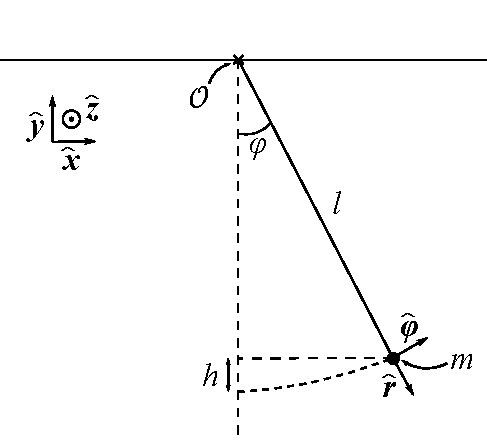
\includegraphics[width=.5\textwidth]{Analytisk-Mekanik/PendulLagrange.pdf}
	\caption{Samme pendul som i afsnit \ref{sec: Beskrivelse af pendul - Newton}. Pendulets højde, $h$, defineres ud fra nulpunktet for den potentielle energi, der vælges til at være pendulets ligevægtspunkt $(0,-l)$ (i kartesiske koordinater).}
	\label{fig:PendulLagrange}
\end{figure}

\noindent
Først kigger vi på pendulet, hvorved vi finder, at dets længde er $l$ og loddet for enden af det har masse $m$. Der defineres et nulpunkt for pendulet, hvor lodet befinder sig, når pendulet er i hvile, altså når det hænger lodret ned (se figur \ref{fig:PendulLagrange}).
Siden der kun er tale om en rotationel bevægelse, vælges et polært koordinatsystem. Den kinetiske energi af pendulet er givet ved
%
\begin{align}
	K &= \frac{1}{2} m v^2 \: ,
\end{align}
%
hvor hastigheden $v$ for en rotationel bevægelse er givet ved pendulets længde $l$ og dets vinkelhastighed $\dt{\phi}$, ligning \eqref{eq:SmartFart}, hvorfor den kinetiske energi bliver
%
\begin{align} \label{Pendul lagrange: Kinetisk energi}
	K &= \frac{1}{2} m (l \dt{\phi})^2 \: .
\end{align}
%
Den potentielle energi er givet ved
%
\begin{align}
	V &= mgh \: ,
\end{align}
%
hvor højden $h$ er givet som pendulets længde fratrukket dets projektion på $y$-aksen
%
\begin{align} \label{Pendul lagrange: Hoejde over nul}
	h &= l - l \cos(\phi) = l(1-\cos(\phi)) \: ,
\end{align}
%
hvorfor den potentielle energi bliver
%
\begin{align} \label{Pendul lagrange: Potentiel energi}
	V &= mgl \left(1-\cos(\phi) \right) \: .
\end{align}
%
I Lagrangefunktionen, ligning \eqref{Lagrange_funktion}, indsættes den kinetiske og den potentielle energi fra henholdsvis ligning \eqref{Pendul lagrange: Kinetisk energi} og ligning \eqref{Pendul lagrange: Potentiel energi}, hvilket giver følgende
%
\begin{align}
	L &= K - V = \frac{1}{2} m l^2 \phi^2 - mgl(1-\cos(\phi)) \: ,
\end{align}
%
hvorved de partielt afledede af Lagrangefunktionen med hensyn til $\phi$ og $\dt{\phi}$ bliver
%
\begin{align}
	\pdif{\phi}{L} &= - mgl \sin(\phi) \: , \label{Pendul Lagrange: Partiel afledede mht phi} \\[.5em]
	\pdif{\dt{\phi}}{L} &= m l^2 \dt{\phi} \: ,
\end{align}
%
og findes den tidsafledte af den sidste ligning fås
%
\begin{align}
	\dif{t}{} \left(\pdif{\dt{\phi}}{L}\right) &= m l^2 \ddt{\phi} \: . \label{Pendul Lagrange: Tidsafledede}
\end{align}
%
Indsættes i Euler-Lagrangeligningen, ligning \eqref{Euler-Lagrange}, den partielt aflede af Lagrangefunktionen med hensyn til $\phi$, ligning \eqref{Pendul Lagrange: Partiel afledede mht phi}, samt den tidsafledede af den partielt afledede af Lagrangefunktionen med hensyn til $\dt{\phi}$, ligning \eqref{Pendul Lagrange: Tidsafledede}, fås følgende:
%
\begin{align}
	\pdif{\phi}{L} &= \dif{t}{} \left(\pdif{\dt{\phi}}{L}\right) \nonumber \\
	\Rightarrow - mgl \sin(\phi) &= m l^2 \ddt{\phi} \: .
\end{align}
%
I ovenstående ligning isoleres vinkelaccelerationen $\ddt{\phi}$
%
\begin{align}
	\ddt{\phi} &= - \frac{g}{l} \sin(\phi) \: .
\end{align}
%
Antages det at pendulets udsving vil være små, da kan der gøres brug af Taylorudviklingen for $\sin(\phi)$, tabel \ref{Taylorseries_table}, hvorved der fås
%
\begin{align}
	\ddt{\phi} &\simeq - \frac{g}{l} \phi \: ,
\end{align}
%
hvilket er pendulligningen, ligning \eqref{eq:PendulLigning}. Hvorfor skulle dette være simplere på denne måde end den Newtonske beskrivelse? Så snart man bliver god til at differentiere rigtig, og opskrive Euler-Lagrangeligningen i nogle gode koordinater, så er denne metode markant lettere at benytte - det er bare et spørgsmål om træning.
%
\subsection{Pendul med rotationel og translatorisk bevægelse} \label{sec:elevator}
%
\begin{figure}[h!]
	\centering
	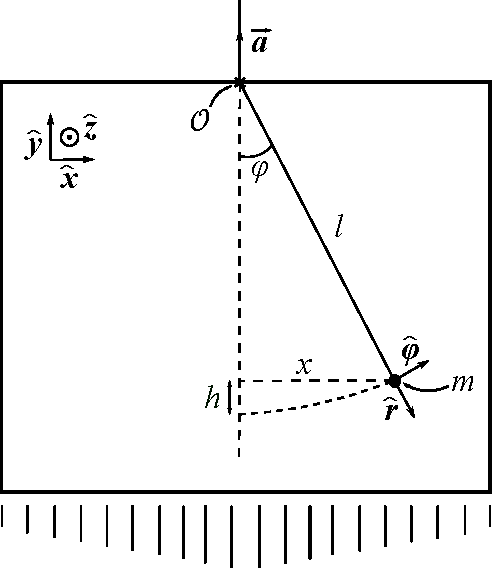
\includegraphics[scale=0.7]{Analytisk-Mekanik/PendulElevator.pdf}
	\caption{Samme pendul som i figur \ref{fig:PendulLagrange}, dog nu placeret i en lineært accelererende elevator.}
	\label{fig:PendulElevator}
\end{figure}
%
Et anden eksempel, hvor der kan gøres brug af Lagrangemekanikken er, når et problem indeholder både translatorisk og rotationel bevægelse, hvilket kan illustreres af et pendul i en elevator, figur \ref{fig:PendulElevator}. Her bevæger lodet i pendulet sig ved en rotationel bevægelse, hvorimens elevatoren bevæger sig med en translatorisk bevægelse, hvilket her er ved konstant acceleration. Først findes koordinaterne, $x$ og $y$, for loddet samt de tidsafledede af disse:
\begin{equation}
	\begin{aligned}
		x &= l \sin(\phi) \: , \\
		\dt{x} &= l \cos(\phi) \dt{\phi} \: , \\
		y &= l \big(1-\cos(\phi) \big) + \frac{1}{2} at^2 \: , \\
		\dt{y} &= l \sin(\phi) \dt{\phi} + at \: ,
	\end{aligned}
\end{equation}
hvor formlen for $y$ fremkommer som kombination af pendulets $y$-koordinat i forhold til elevatoren, ligning \eqref{Pendul lagrange: Hoejde over nul}, og elevatorens stedfunktion
\begin{align}
	y_{elevator}(t) &= \frac{1}{2}at^2 + v_{0,elevator} t + y_{0,elevator} \: ,
\end{align}
hvor $y_{0,elevator} = v_{0,elevator} = 0$ grundet vores valg af koordinatsystem. Dette valg foretages, da det gør $y$-koordinaten nemmere at regne med.

\noindent
Systemets kinetiske og potentielle energi findes herudfra som henholdsvis
%
\begin{align}
	K &= \frac{1}{2} m \left( \dt{x}^2 + \dt{y}^2 \right) \nonumber \\
	&= \frac{1}{2} m \left[ \left( l^2 \cos^2(\phi) \dt{\phi} \right) + \left( l^2 \sin^2(\phi) \dt{\phi} + a^2t^2 + 2 l \sin(\phi) \dt{\phi} a t \right) \right] \nonumber \\
	&= \frac{1}{2} m \left( l^2\phi^2 + a^2t^2 + 2l\sin(\phi)\dt{\phi}at \right) \, ,
\end{align}
%
og
%
\begin{align}
	V &= mgy = mg \left[ l \left( 1 - \cos(\phi) \right) + \frac{1}{2}at^2 \right] \: ,
\end{align}
%
hvorved Lagrangefunktionen bliver
%
\begin{align}
	L &= K-V = \frac{1}{2} m \left( l^2\dt{\phi}^2 + a^2t^2 + 2l\sin(\phi)\dt{\phi}at \right) - mg \left[ l \left( 1 - \cos(\phi) \right) + \frac{1}{2}at^2 \right] \: .
\end{align}
%
De partielt afledede af Lagrangefunktionen i forhold til henholdsvis $\phi$ og $\dt{\phi}$, samt den tidsafledede af sidste findes:
%
\begin{align}
	\pdif{\phi}{L} &= ml\cos(\phi)\dt{\phi}at - mgl\sin(\phi) \: , \\
	\pdif{\dt{\phi}}{L} &= ml^2\dt{\phi} + ml\sin(\phi)at \: , \\
	\dif{t}{} \left(\pdif{\dt{\phi}}{L}\right) &= ml^2\ddt{\phi} + ml\cos(\phi)\dt{\phi}at + ml\sin(\phi)a \: .
\end{align}
%
Indsættes dette i Euler-Lagrangeligningen fås
%
\begin{align}
	\pdif{\phi}{L} &= \dif{t}{}\left( \pdif{\dt{\phi}}{L} \right) \nonumber \\
	 \Rightarrow ml\cos(\phi)\dt{\phi}at - mgl\sin(\phi) &= ml^2\ddt{\phi} + ml\cos(\phi)\dt{\phi}at + ml\sin(\phi)a \: .
\end{align}
%
Heri isoleres vinkelaccelerationen
%
\begin{align}
	\ddt{\phi} &= - \frac{g+a}{l}\sin(\phi) \: ,
\end{align}
%
og antages pendulets udsving at være lille, kan dette Taylorudvikles til
\begin{align}
	\ddt{\phi} &\simeq - \frac{g+a}{l}\phi \: ,
\end{align}
hvilket er på samme form som pendulligningen, hvorfor dette kan ses som et stillestående system med en ændret tyngdeacceleration, $\tilde{g} = g + a$.

\subsection{Karrusel: System uden potentiel energi} \label{sec:Karrusel}
\begin{figure}
	\centering
	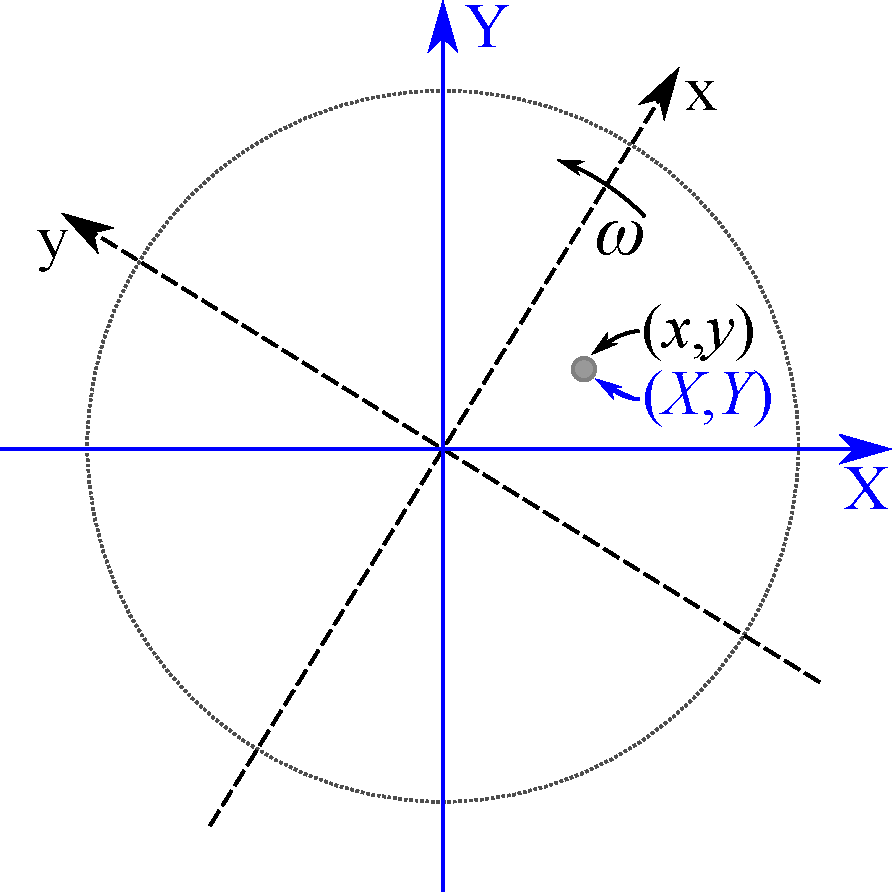
\includegraphics[width=0.4\columnwidth]{Analytisk-Mekanik/Karussel.pdf}
	\caption{Roterende karussel. Det stiplede sorte koordinatsystem roterer med karussellen således, at et punkt på karusellen i dette koordinatsystem altid har koordinaterne $(x,y)$. I det fastlåste blå koordinatsystem roterer karussellen, hvorfor førnævnte punkt i dette koordinatsystem vil have skiftende koordinater, der er givet ved $(X,Y)$, ligning \eqref{eq:Karussel_X_Y_koordinater}.}
	\label{fig:Karussel}
\end{figure}

Ovenfor har der været kigget på systemer, der har haft både kinetisk og potentiel energi, hvorfor der nu ses på et system uden potentiel energi: En karrusel, figur \ref{fig:Karussel}.

\noindent
I dette system betragtes en partikel med masse $m$, der bevæger sig relativt til et roterende koordinatsystem, som følger karrusellen (stiplet koordinatsystem i figur \ref{fig:Karussel}). I dette koordinatsystem har partiklen koordinaterne $(x,y)$. Betragtes dette system ud fra et stillestående koordinatsystem (blåt koordinatsystem i figur \ref{fig:Karussel}) med samme origo, vil karrusellen rotere med en vinkelhastighed $\omega$. I dette koordinatsystem vil partiklens koordinater være $(X,Y)$. Sammenhængen mellem partiklens koordinater i de to koordinatsystemer er givet ved\footnote{Dette fås ved at gange en rotationsmatrix på stedvektoren $\xy{x}{y}$, hvilket her bare tages for gode varer.}
%
\begin{equation} \label{eq:Karussel_X_Y_koordinater}
	\begin{aligned}
		X &= x \cos(\omega t) - y \sin(\omega t) \: , \\
		Y &= x \sin(\omega t) + y \cos(\omega t) \: .
	\end{aligned}
\end{equation}
%
For at finde den kinetiske energi, beregnes de afledede af koordinaterne, hvilket giver
%
\begin{equation}
	\begin{aligned}
		\dt{X} &= \dt{x} \cos(\omega t) - \omega x \sin(\omega t) - \dt{y} \sin(\omega t) - \omega y \cos(\omega t) \: , \\
		\dt{Y} &= \dt{x} \sin(\omega t) + \omega x \cos(\omega t) + \dt{y} \cos(\omega t) - \omega y \sin(\omega t) \: .
	\end{aligned}
\end{equation}
%
Hernæst beregnes summen af de kvadrerede $\dt{X}$- og $\dt{Y}$-koordinater:
%
\begin{align} \label{eq:KarusselHastighed}
	\dt{X}^2 + \dt{Y}^2 &= \dt{x}^2 + \omega^2 x^2 + \dt{y}^2 + \omega^2 y^2 - \dt{x}y \omega + x \dt{y} \omega + x \dt{y} \omega - \dt{x} y \omega \nonumber \\
	&= \dt{x}^2 - \dt{y}^2 + \omega(x^2 + y^2) + 2 \omega (x \dt{y} - \dt{x} y) \: .
\end{align}
%
De første fire led i ligning \eqref{eq:KarusselHastighed} fremkommer på samme måde, og her forklares blot fremkomsten af $\dt{x}^2$ leddet: Kvadreres $\dt{X}$ og $\dt{Y}$ fremkommer led som er kvadrerede, for eksempel
%
\begin{align*}
	[\dt{x} \cos(\omega t)]^2 &= \dt{x}^2 \cos^2(\omega t) \: , \\
	[\dt{x} \sin(\omega t)]^2 &= \dt{x}^2 \sin^2(\omega t) \: .
\end{align*}
%
Siden summen af de kvadredede $\dt{X}$- og $\dt{Y}$-koordinater beregnes, vil man få
\begin{align*}
	\dt{x}^2 \cos^2(\omega t) + \dt{x}^2 \sin^2(\omega t) &= \dt{x}^2 (\cos^2(\omega t) + \sin^2(\omega t)) = \dt{x}^2 \: ,
\end{align*}
%
da $\cos^2(\omega t) + \sin^2(\omega t) = 1$, hvilket kaldes grundrelationen.

\noindent
For de resterende fire led er der også gjort brug af grundrelationen, men her blot mellem krydsleddene: Tages et eksempel kan det ses at
%
\begin{align*}
	\left[\dt{x}\cos(\omega t)\right] \left[-\omega y\cos(\omega t)\right] &= -\dt{x}\omega y \cos^2(\omega t) \: , \\
	\left[\dt{x}\sin(\omega t)\right] \left[-\omega y\sin(\omega t)\right] &= -\dt{x}\omega y \sin^2(\omega t) \: .
\end{align*}
%
Sammenlægges disse to led fås
%
\begin{align*}
	-\dt{x}\omega y \cos^2(\omega t) -\dt{x}\omega y \sin^2(\omega t) &= -\dt{x}\omega y \left(\cos^2(\omega t) + \sin^2(\omega t)\right) = -\dt{x}\omega y \: .
\end{align*}

\noindent
De resterende krydsled fra sammenlægningen $\dt{X}$ og $\dt{Y}$ går ud med hinanden, eksempelvis
%
\begin{align*}
	\left[\dt{x}\cos(\omega t)\right] \left[-\omega x \sin(\omega t)\right] &= -\dt{x}x\omega\cos(\omega t)\sin(\omega t) \: , \\
	\left[\dt{x}\sin(\omega t)\right] \left[\omega x \cos(\omega t)\right] &= \dt{x}x\omega\cos(\omega t)\sin(\omega t) \: ,
\end{align*}
%
hvorfor disse ikke indgår i ligning \eqref{eq:KarusselHastighed}.

\noindent
Ud fra ligning \eqref{eq:KarusselHastighed} fås følgende kinetisk energi
%
\begin{align}
	K &= \frac{1}{2} m \left(\dt{X}^2 + \dt{Y}\right) = \frac{1}{2} m \left[ \dt{x}^2 - \dt{y}^2 + \omega(x^2 + y^2) + 2 \omega (x \dt{y} - \dt{x} y) \right] \: ,
\end{align}
%
og da der ingen potentiel energi er i systemet, bliver Lagrangefunktionen
%
\begin{align}
	L &= K = \frac{1}{2} m \left[ \dt{x}^2 - \dt{y}^2 + \omega(x^2 + y^2) + 2 \omega (x \dt{y} - \dt{x} y) \right] \: .
\end{align}
%
Fra denne Lagrangefunktion kan følgende partielt afledede med hensyn til $x$ og $\dt{x}$ findes
%
\begin{align}
	\pdif{x}{L} &= \frac{1}{2} m \left[ 2\omega^2x + 2\omega \dt{y} \right] = m \left( \omega^2x + \omega \dt{y} \right) \: , \\
	\pdif{\dt{x}}{L} &= \frac{1}{2} m \left[ 2 \dt{x} - 2\omega y \right] = m \left( \dt{x} - \omega y \right) \: , \\
	 \dif{t}{} \left( \pdif{\dt{x}}{L} \right) &= m \left( \ddt{x} - \omega \dt{y} \right) \: ,
\end{align}
%
hvorved Euler-Lagrangeligningen bliver
%
\begin{align}
	\pdif{x}{L} &= \dif{t}{} \left( \pdif{\dt{x}}{L} \right) \nonumber \\
	\Rightarrow m \left( \omega^2 x + \omega \dt{y} \right) &= m \left( \ddt{x} - \omega \dt{y} \right) \: ,
\end{align}
%
så bevægelsesligningen bliver
%
\begin{align} \label{eq:xKarusel}
	\ddt{x} &= \omega^2x + 2 \omega \dt{y} \: .
\end{align}

\noindent
For $y$ og $\dt{y}$ bliver de partielt afledede
%
\begin{align}
	\pdif{y}{L} &= \frac{1}{2} \left[ 2 \omega^2y - 2\omega\dt{x} \right] = m \left( \omega^2y - \omega \dt{x} \right) \: , \\
	\pdif{\dt{y}}{L} &= \frac{1}{2} \left[2 \dt{y} + 2 \omega x \right] = m \left( \dt{y} + \omega x \right) \: , \\
	\dif{t}{} \left(\pdif{\dt{y}}{L}\right) &= m \left( \ddt{y} - \omega \dt{x} \right) \: ,
\end{align}
%
hvorved Euler-Lagrangeligningen bliver
%
\begin{align}
	\pdif{y}{L} &= \dif{t}{} \left(\pdif{\dt{y}}{L}\right) \nonumber \\
	\Rightarrow m \left( \omega^2 y-\omega \dt x \right) &= m \left( \ddt{y} - \omega \dt{x} \right) \: ,
\end{align}
%
og der fås følgende bevægelsesligning for partiklen i $y$-retningen
%
\begin{align} \label{eq:yKarusel}
	\ddt{y} &= \omega^2y - 2 \omega \dt{x} \: .
\end{align}

\noindent
Det kan med nogle lettere bøvlede udregninger vises, at Corioliskraften og centrifugalkraften er givet som
%
\begin{equation} \label{eq:FiktiveKraefter}
\begin{aligned}
	\v{F}_\mathrm{cor} &= 2m\dt{\v{r}}\times\v{\Omega} \: , \\
	\v{F}_\mathrm{cf} &= m(\v{\Omega} \times \v{r}) \times \v{\Omega} \: ,
\end{aligned}
\end{equation}
%
hvor $\v{r}$ er stedvektoren for det legeme, som kræfterne påvirker, og $\v{\Omega}$ er vinkelhastighedsvektoren for det roterende koordinatsystem, som legemet befinder sig i. I dette eksempel roterer karrusellen med vinkelhastigheden $\omega$ omkring $z$-aksen, hvorfor $\v{\Omega} = \omega\zhat$. Enhver vektor kan i kartesiske koordinater skrives på formen $\v{r} = x\xhat + y\yhat + z\zhat$. Af denne grund kan Corioliskraften skrives som
%
\begin{equation}
\begin{aligned}
	\v{F}_\mathrm{cor} &= 2m(\dt{x}\xhat + \dt{y}\yhat + \dt{z}\zhat) \times \omega\zhat \\
	&= 2m\omega(-\dt{x}\yhat + \dt{y}\xhat) \: ,
\end{aligned}
\end{equation}
%
og tilsvarende bliver centrifugalkraften
%
\begin{equation}
\begin{aligned}
	\v{F}_\mathrm{cf} &= m[\omega\zhat \times (x\xhat + y\yhat + z\zhat)] \times \omega\zhat \\
	&= m\omega^2[x\yhat - y\xhat] \times \zhat \\
	&= m\omega^2(x\xhat + y\yhat) \: .
\end{aligned}
\end{equation}
%
Bruges Newtons 2. lov på summen af de fiktive kræfter fås
\begin{align}
	\sum\v{F} &= \v{F}_\mathrm{cor} + \v{F}_\mathrm{cf} \nonumber\\
	\Rightarrow m(\ddt{x}\xhat + \ddt{y}\yhat) &= 2m\omega(-\dt{x}\yhat + \dt{y}\xhat) + m\omega^2(x\xhat + y\yhat) \: ,
\end{align}
%
og samles $x$- og $y$-komposanterne for sig fås
%
\begin{equation}
	\begin{aligned}
		\ddt{x} &= \omega^2x + 2\omega\dt{y} \: , \\
		\ddt{y} &= \omega^2y - 2\omega\dt{x} \: .
	\end{aligned}
\end{equation}
%
Dette er præcis de samme ligninger, som ligningerne \eqref{eq:xKarusel} og \eqref{eq:yKarusel}, hvorfor ovenstående kan tænkes som en pseudoudledning af Coriolis- og centrifugalkraften, og det illustrerer også, at de er effekter, som rotationen skaber fra den kinetiske energi i systemet. Grunden til at det ikke er en rigid udledning er, at den er bundet op på det kartesiske koordinatsystem og én specifik rotation. Karrusellen illustrerer dog eksistensen af disse fiktive kræfter, til en vis grad hvor de kommer fra, og den belyser hvad disse kræfter er for nogle størrelser.


\section{Perspektiver i Analytisk Mekanik}
Euler-Lagrangeligningen giver én andenordens differentialligning for hvert generaliseret koordinat, men disse kan være svære at løse. Nogle gange er det simplere at få to koblede differentialligninger pr. generaliseret koordinat, hvilket kræver en ny formulering af mekanikken.

\subsection{Hamiltonformalismen}
Tankegangen minder meget om den fra Lagrangeformalismen, hvorfor der kan tages udgangspunkt i den til at illustre idéen. Her defineres en Hamiltonfunktion, $H$, af $n$ generaliserede koordinater ud fra Lagrangefunktionen
%
\begin{align} \label{eq:HamiltonDefinition}
	H(q_1,q_2,...,q_n,p_1,p_2,...,p_n,t) \equiv \sum_i^np_i\dt{q}_i - L \: ,
\end{align}
%
hvor $p_i$ er den generaliserede impuls svarende til det $i$'te generaliserede koordinat $q_i$. Det er vigtigt at pointere at en Hamiltonfunktion først kan kaldes en Hamiltonfunktion, når den er udtrykt udelukkende ved de generaliserede stedkoordinater og impulser. Det kommer til at give mening under udledningen af Hamiltons ligninger, der netop er udtrykt ved disse parametre. Den generaliserede impuls er defineret ud fra Lagrangefunktionen som
\begin{align} \label{eq:generaliseretImpuls}
	p_i \equiv \pdif{\dt{q}_i}{L} \: .
\end{align}
I mange tilfælde er Hamiltonfunktionen givet ud fra et systems energier
\begin{align} \label{eq:H=E}
	H = K + V = E \: ,
\end{align}
og den er faktisk ofte systemets samlede energi, hvilket dog ikke uddybes her. \\%, se opgave \ref{opg:HamiltonEnergi}. \\
Differentieres ligning \eqref{eq:HamiltonDefinition} partielt med hensyn til det $i$'te generaliserede koordinat fås
%
\begin{align}
	\pdif{q_i}{H} = p_i\pdif{q_i}{\dt{q}_i} + \pdif{q_i}{p_i}\dt{q_i} - \pdif{q_i}{L} - \pdif{\dt{q}_i}{L}\pdif{q_i}{\dt{q}_i} \: .
\end{align}
%
Alle disse differentialer kommer af at der er tale om en produktfunktion og en sammensat funktion, og man er nød til at tage højde for, at der kan være bidrag fra alle led. Ved brug af ligning \eqref{eq:generaliseretImpuls} ses det, at første og sidste led er ens, men med modsat fortegn. Derudover afhænger $p_i$ ikke eksplicit af $q_i$, hvorfor dens partielt afledte er nul. Dette skyldes at de generaliserede koordinater med tilhørende generaliserede impulser er en komplet basis for systemet, hvilket blandt andet betyder, at ingen af dem kan udtrykkes ved de andre, hvorfor deres partielt afledte med hensyn til hinanden skal være nul. \\
Ved brug af Euler-Lagrangeligningen, ligning \eqref{Euler-Lagrange}, og definitionen på generaliseret impuls, ligning \eqref{eq:generaliseretImpuls}, opnås den første af Hamiltons ligninger:
%
\begin{align}
	\pdif{q_i}{H} = -\pdif{q_i}{L} = -\el{\dt{q_i}} = -\dif{t}{p_i} = -\dt{p_i} \: .
\end{align}
%
Prøves det nu at opskrive den partielt afledede af Hamiltonfunktionen med hensyn til den generaliserede impuls fås
%
\begin{align}
	\pdif{p_i}{H} = p_i\pdif{p_i}{\dt{q}_i} + \pdif{p_i}{p_i}\dt{q_i} - \pdif{p_i}{L} - \pdif{\dt{q}_i}{L}\pdif{p_i}{\dt{q}_i} \: .
\end{align}
%
Pr. definition er Lagrangefunktionen en funktion at de generaliserede koordinater og disses afledte, hvorfor $\partial L/\partial p_i = 0$. Med henvisning til ligning \eqref{eq:generaliseretImpuls} ses det også, at første og sidste led er ens, og da den partielt afledte af en funktion med hensyn til sig selv er 1, fås det at
%
\begin{align}
	\pdif{p_i}{H} = \pdif{p_i}{p_i}\dt{q_i} =  \dt{q}_i \: .
\end{align}
%
Dette er Hamiltons 2. ligning, og skrives de to op sammen er det
%
\begin{equation}
\begin{aligned}
	\pdif{q_i}{H} &=  -\dt{p}_i \: , \\
	\pdif{p_i}{H} &=  \dt{q}_i \: .
\end{aligned}
\end{equation}
%
Her vil der ikke gås i detaljen med, hvorfor Hamiltonformalismen kan være smart sammenlignet med Lagrangeformalismen, og det virker da også umiddelbart som ekstra arbejde, at skulle omskrive Lagrangefunktionen til en gyldig Hamiltonfunktion og så indsætte i Hamiltons ligninger, når man bare kunne have indsat i Euler-Lagrangeligningen. Her må man som læser bare stole på, at der eksisterer tilfælde, hvor Hamiltonformalismen er nemmere at benytte. Et mindre flyvsk argument for at introducere Hamiltonformalismen er dog at kvantemekanikken bygger på netop dette, hvilket ses i form af Hamiltonoperatoren, og alt dette introduceres i kapitel \ref{cha:Kvant} om netop kvantemekanik.

% Herfra overlades det sidste til EHK at finde et hjem for =)

%\subsection{Fra klassisk mekanik til kvantemekanik}
%Kvantemekanikken bygger dog på Hamiltonformalismen, hvorfor idéen med dette afsnit er at introducere Hamiltonfunktionen, der omskrives til Hamiltonoperatoren, $\op{H}$, som kan betragtes som grundstenen for kvantemekanikken, fordi den tidsuafhængige eller stationære Schrödingerligning kan skrives som egenværdiproblemet
%
%\begin{align}
%	\op{H}\psi = E\psi
%\end{align}
%
%Her går $\psi$'erne ikke ud med hinanden, da dette er formuleret ved hjælp af den gren af matematikken, der hedder lineær algebra, hvilket gør matematikken meget lettere, når først man har styr på denne disciplin. Det er dog meget abstrakt at lære, hvorfor det ikke vil beskrives detaljeret her. Hamiltonoperatoren kan opskrives ud fra den klassiske Hamiltonfunktion ved at benytte at kinetisk energi kan udtrykkes på følgende måde for et generaliseret koordinat
%
%\begin{align} \label{eq:K(p)}
%	K =  \frac{p^2}{2m}
%\end{align}
%
%hvilket kan motiveres ved at den generaliserede impuls ofte kan skrives på formen $p = m\dt{q}$, som giver definitionen på kinetisk energi, ved indsættelse i ligning \eqref{eq:K(p)}. Derved giver ligning \eqref{eq:H=E} at
%
%\begin{align}
%	H = K + V = \frac{p^2}{2m} + V
%\end{align}
%
%som på operatorform er
%
%\begin{align}
%	\op{H} = \frac{\op{p}^2}{2m} + V
%\end{align}
%
%Benyttes impulsoperatoren i tabel \ref{tab:operatorer_i_kvant} nu, samt definitionen på tallet $i$, nemlig at $i^2 = -1$ fås hamiltonoperatoren fra samme tabel
%
%\begin{align}
%	\op{p}^2 &= \left(-i\hbar\pdif{x}{}\right)^2 = \hbar^2\pdif[2]{x}{} \\
%	\op{H} &= \frac{\op{p}^2}{2m} + V = -\frac{\hbar^2}{2m}\pdif[2]{x}{} + V
%\end{align}
%
%Der er hermed dannet en bro mellem klassisk mekanik og kvantemekanik, og målet med dette er at vise at en sådan bro eksisterer fremfor en rigid gennemgang af Hamiltonformalismen og dens klassiske mangfoldigheder. \\

%Konkluderende kan det siges at metoden til at analysere et kvantemekanisk system er at opskrive systemets kinetiske og potentielle energi, for derefter at opstille systemets Hamiltonfunktion. Denne omskrives til en Hamiltonoperator, som giver mening for systemet, og derefter løses den stationære Schrödingerligning. Dette kan lyde relativt simpelt, men der kan komme en del komplikationer i forbindelse med eksempelvis skridtet med at omskrive Hamiltonfunktionen til en passende Hamiltonoperator.